\documentclass{article}
\usepackage{iclr2027_conference,times}
\usepackage{amsmath,amssymb,booktabs,graphicx,microtype,multirow,float}
\usepackage{hyperref}
\usepackage{url}

\newcommand{\M}{\ensuremath{M}}
\newcommand{\Mp}{\ensuremath{M'}}
\newcommand{\gain}{\ensuremath{\Delta}}
\newcommand{\zscore}{\ensuremath{z_{\mathrm{pc}}}}

\title{Should This Concept Enter Memory?\\
Placebo-Calibrated Predictive Compression at Inference Time}

\author{Anonymous Authors}

\begin{document}
\maketitle

\begin{abstract}
When a user teaches a language model a novel term, a persistent-memory system must decide
whether the model inferred the intended meaning before saving it. Existing write gates score
confidence, consistency, novelty, or source trust; each can approve a confident, self-consistent
misreading. We instead ask whether a candidate meaning compresses the user's subsequent usage.
For each candidate, we measure held-out usage log-loss reduction and standardize it against six
surface-matched placebo meanings. We introduce \emph{gavagai pairs}: teaching sets on which the
intended meaning and a tempting misreading are extensionally identical, followed by usage that
separates them. In a confirmatory test fixed before model evaluation (90 primary pairs, five unseen
generator seeds), placebo-calibrated gain distinguishes the intended meaning from the misreading
with AUC $0.949$ (95\% hierarchical bootstrap CI $[0.916,0.977]$) on Qwen2.5-1.5B and
$0.909$ $[0.860,0.955]$ on Qwen2.5-3B, and $0.811$ $[0.740,0.878]$ on the held-out
SmolLM2 family. A ConsistencyGate-style support score obtains $0.370$, $0.440$, and $0.581$;
semantic entropy obtains $0.230$, $0.249$, and $0.439$. A threshold selected only on development
data transfers to unseen items with 55.6\% true-concept admission at 9.5\% all-negative false
admission on the 1.5B model, but requires model-specific recalibration at 3B. In an end-to-end
stress test, writing the first generated candidate hurts held-out log loss by $2.28$ nats on average,
whereas admitted candidates improve it by $1.44$ nats with 92\% precision at 27.8\% coverage.
Crucially, six observations do not repay a full textual description code on any test item; our
result supports predictive compression as an admission signal, not a claim of immediate two-part
MDL payback. Code, frozen splits, and every failed condition are included.
\end{abstract}

\section{Introduction}

Suppose a user says that a yellow wooden bowl is \emph{dax}, and later that a yellow metal cup is
also \emph{dax}. Did \emph{dax} mean yellow, wooden, bowl, or some conjunction? A model can be
confident in the wrong answer because the teaching examples do not distinguish these hypotheses.
If a persistent-memory system writes the first plausible interpretation, the error outlives the
conversation and may become harder to correct.

We study the decision immediately before such a write. The model has inferred one or more candidate
meanings from a teaching interaction and then observes a small buffer of the same interlocutor's
subsequent uses. No answer key says what the word means. The gate must accept a candidate, reject it,
or wait for more evidence. The desired signal is therefore not whether the model already endorses
the candidate, but whether the candidate predicts the user's behavior better than reasonable
alternatives.

Prediction and compression give a simple operational test: the reduction in log loss after
conditioning on a candidate is exactly the number of nats it saves when coding the observed usage
\citep{deletang2024compression,cover1999elements}. Yet raw predictive gain is poorly calibrated
across items: some definitions are easy for the base model to follow, while others barely change its
predictions. We standardize each candidate against six automatically constructed placebo meanings.
The resulting score, \zscore{}, asks whether the candidate compresses usage unusually well for
\emph{this item}, rather than whether its raw gain exceeds a global scale-dependent number.

Evaluating this question requires ambiguity by construction. Ordinary concept-learning benchmarks
usually reveal the intended label in their examples; then a confident-support score is often enough.
Our \emph{gavagai pairs} instead provide a true meaning \M{} and a tempting misreading \Mp{} that
make identical predictions on every teaching example. Only later uses separate them. Ground truth is
available to the evaluator but never to the gate. This creates the precise failure mode that a
persistent write policy must survive: a hypothesis can be novel, simple, highly supported, and wrong.

Our contributions are:
\begin{enumerate}
  \item a controlled benchmark of five ambiguity families, with a frozen confirmatory split across
  five unseen generator seeds and explicit scope diagnostics;
  \item a placebo-calibrated predictive-compression score and development-only admission protocol,
  evaluated against direct support, entropy, surprise, simplicity, and raw-gain baselines; and
  \item an end-to-end stress test that extracts usage decisions from natural utterances, samples
  candidate definitions, and applies the frozen gate before evaluation.
\end{enumerate}
We also report three negative results that materially narrow the claim. A threshold does not transfer
unchanged across model scales; relational meanings are outside the reliable scope of the tested base
models; and the predictive savings from six observations never repay a full textual description.

\section{Related work}

\paragraph{Persistent memory and write gates.}
Context distillation, adapters, and trained prefixes can turn contextual information into reusable
state \citep{snell2022distilling,chen2024generativeadapter,eyuboglu2025cartridges}. The orthogonal
question is what should be admitted. Continual-learning and agent-memory systems gate writes using
randomness or representativeness, geometric novelty, normalized loss, Bayesian surprise, and source
trust \citep{prabhu2020gdumb,aljundi2019gss,wang2026sage,li2025selfsizing,
gorlo2026worth,zahn2026writetime,yang2026trustmem}. These signals answer whether an item is useful,
new, or trustworthy, not whether a candidate interpretation predicts the teacher's later usage.

The closest locus is ConsistencyGate \citep{zhang2026consistencygate}, which places a
ground-truth-free gate before an inference-time persistent write. Consensus gates also filter
self-training data \citep{huang2022selfimprove,stein2026gates}. Our novelty claim is therefore only
about the \emph{criterion}: held-out predictive compression relative to item-matched placebos. We
implement the latency-oriented support probability of ConsistencyGate as a direct baseline.

\paragraph{Uncertainty and compression.}
Semantic entropy detects inconsistent generations \citep{farquhar2024semantic}, but an
over-specific misreading can be both wrong and low-entropy. Agreement is likewise not a standalone
correctness certificate \citep{ding2026agree}. Rate--distortion views of agent memory ask what to
retain under a budget or how to preserve the agent's own decisions
\citep{colaco2026ratedistortion,zou2026demem}. We instead score a candidate before it is written and
use another party's later word choices as evidence. We test both predictive savings and explicit
two-part codes, and keep their conclusions separate.

\section{Method}
\label{sec:method}

\subsection{Predictive compression from later usage}

For one interlocutor and novel word, let $T$ be teaching examples and let $c$ be a candidate meaning
induced from $T$. After induction, the system buffers $n$ later usage events
$D=\{(x_j,y_j)\}_{j=1}^{n}$, where $y_j\in\{0,1\}$ indicates whether the interlocutor applies the
word to $x_j$. Let $q_0(y\mid x,T)$ be the base prediction and $q_c(y\mid x,T,c)$ the prediction when
conditioned on $c$. The predictive compression gain is
\begin{equation}
\gain(c;D)=\operatorname{NLL}_{0}(D)-\operatorname{NLL}_{c}(D)
=\sum_{j=1}^{n}\log\frac{q_c(y_j\mid x_j,T,c)}{q_0(y_j\mid x_j,T)}.
\label{eq:gain}
\end{equation}
Positive gain means the candidate shortens a prequential code for observed usage. The buffer is
temporally later than induction but earlier than persistent consolidation; deploying the gate thus
trades immediate writing for evidence.

\subsection{Item-matched placebo calibration}

Raw gain depends on prompt sensitivity and the model's ability to follow a definition. For each item
we automatically generate $K=6$ placebo candidates: two wrong atomic meanings, one wrong
conjunction, two over-specific meanings, and one over-broad meaning. They match the surface form and
complexity range of plausible hypotheses without inspecting the true meaning. Let $\mu_i$ and $s_i$
be the sample mean and standard deviation of their gains. Our primary score is
\begin{equation}
\zscore(c)=\frac{\gain(c)-\mu_i}{s_i}.
\label{eq:z}
\end{equation}
On development data only, we select a single acceptance threshold that maximizes true-candidate
admission subject to false admission of \Mp{} and placebos not exceeding 10\%. The threshold is then
frozen. This is a selective policy: low coverage is acceptable if admitted candidates are reliable.

\paragraph{Not all compression scores are two-part MDL.}
Equation~\ref{eq:gain} is predictive code savings, and Equation~\ref{eq:z} is a calibrated signal;
neither subtracts the cost of specifying $c$. We separately evaluate
$G_L(c)=\gain(c)-L(c)$ using (i) an index into the shared candidate pool, (ii) the reference model's
NLL for the textual statement, and (iii) a fixed-width token code. We call a concept ``paid for''
only when the corresponding $G_L>0$.

\subsection{Baselines}

All scores see the same candidate pairs. \emph{Support} is the model probability that a candidate is
consistent with all teaching examples, matching the single-pass log-probability form of
ConsistencyGate. \emph{Semantic entropy} is negative mean Bernoulli entropy of conditioned held-out
usage predictions. \emph{Surprise} is mean Bernoulli KL divergence from the no-definition
predictions. \emph{Simplicity} is negative reference-model description length. We also report raw
gain $\gain$ and the best-placebo margin. Appendix~\ref{app:prompts} gives exact prompts.

\section{Experimental design}
\label{sec:setup}

\subsection{Gavagai pairs}

Each item contains a pseudoword, six teaching examples, an intended meaning \M{}, a misreading
\Mp{}, six placebo meanings, and three to six held-out uses. By construction, \M{} and \Mp{} label
every teaching example identically and disagree on held-out examples. The primary domain contains:
(G1) an atomic property versus a conjunction; (G2) a superordinate category versus the single
observed kind; and (G3) a material versus a perfectly correlated object kind. G4 tests argument
order and G5 absolute versus relative size. Pilot experiments, conducted before the confirmatory
split, showed unreliable definition following on G4 and prior override on G5; we therefore declared
G1--G3 primary and retained G4--G5 as scope diagnostics.

Table~\ref{tab:example} illustrates why ordinary validation on teaching examples is insufficient.
Both candidates achieve perfect teaching accuracy, and the conjunction may receive higher support
because every positive happens to be wooden. The later yellow metal object supplies the information
that the teaching set lacks. Placebos are generated from fixed templates (for example, \emph{red},
\emph{wooden}, \emph{yellow and shiny}, and \emph{a thing}) rather than chosen after scoring.

\begin{table}[t]
\caption{Schematic G1 gavagai pair. The gate observes the teaching set and later usage, but never the
evaluator-only names \M{} and \Mp{}.}
\label{tab:example}
\centering\small
\setlength{\tabcolsep}{5pt}
\begin{tabular}{lllcc}
\toprule
stage & described object & Tovi says \emph{dax}? & \M{}: yellow & \Mp{}: yellow $\wedge$ wooden \\
\midrule
teaching & yellow wooden bowl & yes & yes & yes \\
teaching & yellow wooden cup & yes & yes & yes \\
teaching & red metal bowl & no & no & no \\
later & yellow metal cup & yes & yes & \textbf{no} \\
later & red wooden cup & no & no & no \\
\bottomrule
\end{tabular}
\end{table}

The development set is the existing seed-11 set (40 items, eight per family). The frozen test uses
five unseen seeds $\{101,211,307,401,503\}$, six items per family and seed: 150 items total, of which
90 are primary. Test examples were not inspected when selecting thresholds. We evaluate canonical
and dictionary-style definition prompts. The frozen models are Qwen2.5-1.5B-Instruct,
Qwen2.5-3B-Instruct, and SmolLM2-1.7B-Instruct; all are used without parameter updates. The 1.5B
Qwen model alone selects thresholds.

\subsection{Statistics and contamination control}

The primary comparison is \M{} versus \Mp{} on unseen G1--G3 items. We report pooled AUC, paired
wins, a one-sided sign test fixed before evaluation, and 95\% hierarchical bootstrap intervals that
resample generator seeds and then items within a seed. Every prompt, model, seed, and failed family
is retained. All-negative false-admission includes \Mp{} and all placebos, preventing a relative
ranking metric from hiding a gate that always accepts something. Before teaching, the model also
scores held-out labels using each pseudoword alone; near-chance AUC and tokenization statistics test
for accidental pretraining associations.

\subsection{End-to-end interface stress test}

P12 supplies candidate meanings and structured usage labels to isolate the admission criterion. P13
adds two interfaces. First, each usage decision is rendered as one of four natural utterance
templates; a probability threshold selected on development utterances extracts whether the speaker
applies the word. Second, the 1.5B model samples four concise candidate definitions from teaching
examples only. The gate selects the candidate with largest \zscore{} and accepts it only at P12's
frozen threshold. Evaluation uses true labels only afterward. The frozen primary generation seed is
reported separately from two explicitly post-hoc decoding-seed checks. This remains a templated
microworld stress test, not a natural-conversation benchmark.

\section{Results}
\label{sec:results}

\subsection{Predictive compression separates intended meanings}

On 90 unseen primary pairs, \zscore{} reaches AUC $0.949$ on Qwen2.5-1.5B and $0.909$ on 3B
(Table~\ref{tab:main}); paired wins are $87/90$ ($p=9.82\times10^{-23}$) and $80/90$
($p=5.26\times10^{-15}$). Performance is not driven by one generator seed: 1.5B canonical AUC is
$0.926$--$0.975$ across the five seeds, with 17 or 18 wins out of 18 in each. A dictionary-style
prompt yields $0.968$ and $0.893$, so the signal is not tied to the canonical wording.
On the held-out SmolLM2 family, canonical AUC is $0.811$ ($[0.740,0.878]$, 74/90 wins,
$p=2.19\times10^{-10}$); changing only to the predeclared dictionary prompt improves it to
$0.912$ $[0.828,0.973]$. The cross-family effect is therefore positive but more prompt-sensitive.

\begin{table}[t]
\caption{Unseen G1--G3 test, canonical prompt. Intervals hierarchically resample generator seeds and
items. Support is the direct ConsistencyGate-style baseline. SmolLM results are filled by the same
frozen protocol and never used for calibration.}
\label{tab:main}
\centering
\small
\setlength{\tabcolsep}{3.4pt}
\begin{tabular}{lccccc}
\toprule
Model & placebo-$z$ & raw gain & support & sem. entropy & surprise \\
\midrule
Qwen2.5-1.5B & \textbf{.949} [.916,.977] & .874 & .370 & .230 & .526 \\
Qwen2.5-3B   & \textbf{.909} [.860,.955] & .851 & .440 & .249 & .732 \\
SmolLM2-1.7B & \textbf{.811} [.740,.878] & .662 & .581 & .439 & .580 \\
\bottomrule
\end{tabular}
\end{table}

The direct baselines clarify the mechanism. Support is below chance on both Qwen scales because the
narrower misreading is fully consistent with teaching and often easier to endorse. Semantic entropy
is more strongly inverted: confidence rewards the over-specific interpretation. Surprise improves
at 3B but remains below calibrated gain. Simplicity reaches $0.751$ at 1.5B (Appendix
Table~\ref{tab:all-scores}); it captures part of the atomic-versus-conjunctive structure but cannot
resolve the material--kind family. Figure~\ref{fig:confirmatory} summarizes these comparisons.

Placebo calibration, rather than predictive loss alone, accounts for a substantial part of the
improvement: at 1.5B, raw gain obtains $0.874$, subtracting the best placebo obtains $0.943$, and
standardizing by the placebo distribution obtains $0.949$. The placebos measure whether a particular
prompt/model pair can express the hypothesized distinction on that item. This also explains the hard
boundary on G4 below: when all definitions fail to control predictions, normalization cannot create
missing conditional behavior.

\begin{figure}[t]
  \centering
  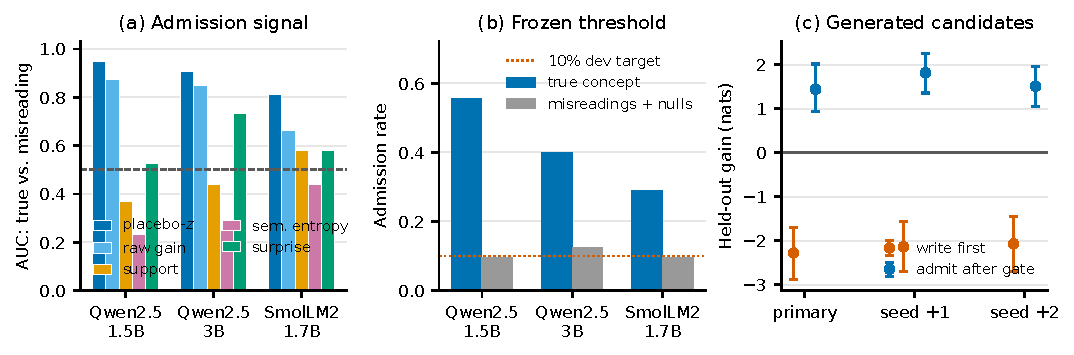
\includegraphics[width=\linewidth]{figures/fig_confirmatory.pdf}
  \caption{(a) Direct baselines on unseen candidate pairs. Dashed line is chance. (b) One admission
  threshold selected on 1.5B development data and applied without retuning. (c) End-to-end generated
  candidates: first-candidate write-all versus candidates admitted by the frozen gate; bars are 95\%
  item-bootstrap intervals. The first seed is confirmatory; the other two are post-hoc robustness.}
  \label{fig:confirmatory}
\end{figure}

\subsection{A development-frozen threshold works within scale, not across scales}

The development rule chooses $\zscore>1.143$ (development TPR 50.0\%, FPR 9.5\%). On unseen 1.5B
canonical items it admits 55.6\% of true meanings, 3.3\% of misreadings, and 10.6\% of placebos; the
combined all-negative FPR is 9.5\%. Under the dictionary prompt, the corresponding rates are 47.8\%
and 8.9\%. Thus the frozen threshold transfers across items and prompt wording at the development
model scale.

At 3B, true admission falls to 40.0\% and all-negative FPR rises to 12.4\%. More importantly, a
development-selected absolute ``decidability'' threshold retains 67.8\% of 1.5B pairs at 98.4\%
pair accuracy but retains none at 3B. A dimensionless score does not guarantee cross-model
calibration: deployment requires calibration data for each base model. We therefore retract the
earlier cross-scale threshold claim and treat AUC, not a universal threshold, as the cross-model
result.
On SmolLM2, the same canonical threshold preserves the intended error rate (9.7\% all-negative FPR)
but admits only 28.9\% of true meanings; the dictionary prompt yields 57.8\% TPR and 8.9\% FPR.
Thus a conservative threshold can transfer accidentally well in error rate while its operating
coverage remains model- and prompt-dependent.

\subsection{Predictive savings do not repay a textual definition in six uses}

Subtracting the shared candidate-index cost yields positive net gain for 47.8\% of true 1.5B
candidates and 65.6\% at 3B. In contrast, neither the reference-model text code nor the fixed-width
text code is repaid by any true candidate. For items with positive predictive gain, a stationary-use
extrapolation gives a median text-code payback horizon of 84.3 observations (IQR 60.3--132.7) at
1.5B, 38.6 (19.6--105.4) at 3B, and 339.5 (187.9--558.4) on SmolLM2. This extrapolation is not observed future performance. The
supported claim is that predictive gain identifies the better hypothesis; whether it is economical
to store a full natural-language definition depends on representation cost and expected future use.

\subsection{Generated candidates turn write-all loss into selective gain}

Natural-utterance extraction obtains AUC $0.99996$ and 99.38\% accuracy on 480 unseen utterances,
using a threshold chosen on 128 development utterances. This near-ceiling result reflects explicit
affirmative/rejection templates and should not be read as open-domain semantic parsing.

The candidate generator is substantially less reliable, which makes the admission decision
meaningful. In the frozen run, writing its first definition decreases held-out compression gain by
$2.278$ nats on average (95\% item-bootstrap CI $[-2.877,-1.701]$). The frozen gate admits 25 of 90
items (27.8\% coverage); 23 of 25 admitted candidates are beneficial (92.0\% precision), and their
mean gain is $+1.441$ nats $[+0.935,+2.017]$. Across two post-hoc decoding seeds, coverage is
32.2--35.6\%, precision 87.5--93.1\%, write-all gain $-2.136$ to $-2.069$, and admitted gain
$+1.510$ to $+1.818$. Selection regret versus the best of four candidates is at most 0.001 nats on
average because extracted labels are almost exact; candidate quality, not selection among candidates,
is the current bottleneck.

\subsection{Scope and contamination}

The declared G4 argument-order diagnostic is at chance (1.5B AUC $0.559$, 95\% CI
$[0.454,0.673]$), showing that compression cannot rescue a model that does not condition on the
candidate definition. G5 reaches $0.849$ but is excluded from the primary claim because pilots
revealed prior override. Before teaching, the pseudowords alone do not separate primary labels:
per-family AUC is $0.510$--$0.533$ at 1.5B and $0.454$--$0.531$ at 3B. Only 3.3\% of pseudowords are
single tokens (mean 2.2 tokens per word). On SmolLM2, primary-family zero-shot AUC is
$0.500$--$0.508$ and only 0.7\% are single tokens. Its G5 zero-shot AUC is $0.946$, however, and its
post-definition G5 candidate AUC is inverted at $0.261$; both were retained as declared diagnostics
and further support excluding G5 from the primary claim. These controls make memorized word meanings an implausible
explanation, while not proving absence from all pretraining data.

\paragraph{Error analysis.}
All three 1.5B pairwise errors occur in G2 category-level ambiguities: two \emph{stick} versus
\emph{cane} items and one \emph{toy} versus \emph{kite} item. Their score gaps are small
($0.01$--$0.35$), but one has high base decidability, showing that uncertainty alone would not catch
every semantic error. The two harmful P13 admissions are also G2. Both generated descriptions are
over-specific (a kite-like object and a neck-worn textile), and both lie near the frozen threshold
($z=1.57$ and $1.20$). More diverse negative placebos or a minimum absolute-gain condition are
promising, but tuning them on these errors would invalidate the confirmation; we leave them as future
hypotheses.

\section{Limitations and implications}

The study uses small instruction-tuned models, English prompts, a finite symbolic microworld, and
binary usage decisions. Its strongest evidence is for choosing between supplied hypotheses; P13's
generated candidates remain templated and low-coverage. Natural conversation may contain indirect,
pragmatic, drifting, or strategically misleading usage. The method also needs later observations,
so it cannot validate a concept immediately after a single explanation.

Predictive fit is not truth. The gate estimates an interlocutor-specific convention, including a
stable false belief; source trust and safety policies remain separate layers. Repeated evaluation on
the same buffer may overfit candidate search, requiring a fresh validation suffix or sequential
testing in longer interactions. A real memory system must additionally enforce per-user isolation,
deletion, privacy, and correction. Appendix~\ref{app:substrate} summarizes our storage experiments;
they show why admission and representation should be evaluated separately.

Despite these limits, the negative results point to a practical design. Buffer evidence; compare
multiple induced hypotheses using future usage; calibrate against matched placebos; abstain by
default; encode frequently reused concepts compactly; and recalibrate whenever the base model or
prompting interface changes.

\section{Conclusion}

A confident interpretation is not necessarily one worth writing. On controlled ambiguities,
placebo-calibrated predictive compression distinguishes intended meanings from self-consistent
misreadings where support and entropy fail, and it converts harmful write-all candidate generation
into a selective positive-gain policy. The result is narrower than immediate MDL consolidation:
full textual descriptions do not repay their code cost in six uses, and thresholds are model
specific. That separation---predictive evidence first, storage economics second---is the central
lesson for inference-time concept memory.

\paragraph{Reproducibility statement.}
The repository includes the frozen protocol timestamped before confirmatory evaluation, deterministic
data generators and exact splits, all prompts, raw per-item probabilities and scores, development-only
threshold selection, hierarchical-bootstrap code, environment versions, and negative conditions. No
API or proprietary model is required. Appendix~\ref{app:repro} lists commands and artifact paths.

\paragraph{LLM usage disclosure.}
An OpenAI Codex model assisted substantially with experiment implementation and orchestration,
statistical analysis code, figure generation, literature organization, and manuscript drafting. The
human authors directed the research questions and are responsible for independently inspecting the
code, verifying the reported artifacts, validating citations and claims, and approving the submitted
manuscript.

\bibliography{refs}
\bibliographystyle{iclr2027_conference}

\appendix
\raggedbottom

\section{Exact prompts and scores}
\label{app:prompts}

For candidate $c$, the canonical definition prefix is ``In Tovi's usage, [word] means [meaning].''
The dictionary variant is ``Tovi's dictionary entry: [word] --- [meaning].'' Each observation then
asks whether Tovi would apply the word to the described object and scores the next-token probabilities
of \texttt{Yes} and \texttt{No}, renormalized over those two tokens. The base condition states only
that the word is unfamiliar. Support receives the teaching examples and candidate statement and asks
whether the meaning is consistent with every example. P13 induction asks for one concise
dictionary-style meaning consistent with all teaching examples and samples four sequences at
temperature 0.8, top-$p$ 0.9, capped at 18 new tokens.

\begin{table}[H]
\caption{All primary pair scores, Qwen2.5 canonical prompt. AUC compares \M{} against \Mp{}.}
\label{tab:all-scores}
\centering\small
\begin{tabular}{lrrrrrr}
\toprule
Score & \multicolumn{2}{c}{Qwen 1.5B} & \multicolumn{2}{c}{Qwen 3B} & \multicolumn{2}{c}{SmolLM 1.7B} \\
 & AUC & wins & AUC & wins & AUC & wins \\
\midrule
placebo-$z$ & .949 & 87/90 & .909 & 80/90 & .811 & 74/90 \\
raw gain & .874 & 87/90 & .851 & 80/90 & .662 & 74/90 \\
best-placebo margin & .943 & 87/90 & .810 & 80/90 & .769 & 74/90 \\
model-text net gain & .918 & 89/90 & .882 & 86/90 & .758 & 76/90 \\
support & .370 & 35/88 & .440 & 43/89 & .581 & 43/76 \\
semantic entropy & .230 & 18/90 & .249 & 13/90 & .439 & 29/90 \\
surprise & .526 & 51/90 & .732 & 68/90 & .580 & 57/90 \\
simplicity & .751 & 74/90 & .779 & 80/90 & .741 & 74/90 \\
\bottomrule
\end{tabular}
\end{table}

\section{Frozen protocol and additional results}

The confirmatory protocol was written before any P12 model run. Development uses generator seed 11.
Test uses seeds 101, 211, 307, 401, and 503. The direction of the sign test, primary G1--G3 domain,
two prompt variants, three models, all-negative FPR, code-length definitions, and interpretation
rules were fixed in advance. The rules explicitly require removal of cross-family or two-part-MDL
claims if the corresponding tests fail.

\begin{table}[H]
\caption{Frozen-threshold unseen-test admission. The threshold is selected only on Qwen2.5-1.5B
canonical development data. ``Neg.'' pools \Mp{} and six placebos.}
\centering\small
\begin{tabular}{llrrrr}
\toprule
Model & prompt & \M{} TPR & \Mp{} FPR & placebo FPR & all-neg. FPR \\
\midrule
Qwen2.5-1.5B & canonical & .556 & .033 & .106 & .095 \\
Qwen2.5-1.5B & dictionary & .478 & .033 & .098 & .089 \\
Qwen2.5-3B & canonical & .400 & .000 & .144 & .124 \\
Qwen2.5-3B & dictionary & .456 & .011 & .146 & .127 \\
SmolLM2-1.7B & canonical & .289 & .056 & .104 & .097 \\
SmolLM2-1.7B & dictionary & .578 & .022 & .100 & .089 \\
\bottomrule
\end{tabular}
\end{table}

\begin{table}[H]
\caption{Canonical placebo-$z$ by primary ambiguity family on Qwen2.5-1.5B.}
\centering\small
\begin{tabular}{lrrr}
\toprule
Family & $n$ & AUC [95\% hierarchical CI] & paired wins \\
\midrule
G1 atomic vs. conjunction & 30 & .950 [.874,1.000] & 30/30 \\
G2 category vs. kind & 30 & .937 [.849,.984] & 27/30 \\
G3 material vs. kind & 30 & 1.000 [1.000,1.000] & 30/30 \\
\bottomrule
\end{tabular}
\end{table}

\section{Admission-signal taxonomy}

\begin{table}[H]
\caption{Representative write or consolidation signals. Our distinction is the criterion, not the
existence or inference-time locus of a gate.}
\centering\small
\begin{tabular}{p{.22\linewidth}p{.39\linewidth}p{.25\linewidth}}
\toprule
Family & signal & typical locus \\
\midrule
GDumb / reservoir & randomness or class balance & replay write \\
GSS / MIR & gradient diversity or interference & replay write/retrieval \\
SAGE & geometric novelty & online write \\
Self-Sizing Hopfield & normalized-loss hysteresis & online write \\
Worth Remembering & Bayesian surprise & online write \\
Write-Time Gating / TRUSTMEM & source trust or faithfulness & agent-memory write \\
GATES / LMSI & sampled self-consistency & training-data admission \\
ConsistencyGate & candidate support probability & inference-time persistent write \\
DeMem & rate--distortion of agent decisions & budgeted compaction \\
Ours & held-out user-usage compression vs. placebos & inference-time persistent write \\
\bottomrule
\end{tabular}
\end{table}

\section{Storage substrate boundary}
\label{app:substrate}

Separate pilot experiments (P3--P11) tested whether context-derived behavior could be stored in a
small per-user parameter delta. Deltas persisted and were isolated by user identifier, but a
word-substitution control showed that the strongest delta stored a word-independent bias over
objects rather than a lexical binding: replacing the taught pseudoword with an opposite-meaning word
barely changed its effect. Token-triggered lexical entries restored binding but lost part of the
cross-format transfer of context injection. We therefore do not present the substrate as concept
learning and do not use it in the admission results. The lesson is methodological: persistence,
partition isolation, lexical binding, and transfer need separate controls.

\section{Reproduction}
\label{app:repro}

From \texttt{research/learning-in-referencing}, create the pinned environment in
\texttt{requirements.txt}. Then run \texttt{p12/generate\_splits.py}, one invocation of
\texttt{p12/eval\_gate.py --model MODEL} per listed model,
\texttt{p12/contamination.py --model MODEL}, and \texttt{p12/analyze.py}. Run
\texttt{p13/run\_endtoend.py} for the frozen seed and listed robustness seeds, followed by
\texttt{p13/analyze.py}. Figure data are regenerated by
\texttt{paper/figures/make\_iclr\_figures.py}. Raw JSON retains every item, candidate, score, model,
prompt variant, split, and generator seed.

\end{document}
